\begin{frame}
    \begin{PointSix}{Learning Goals}
      \alert{Learning goals today:}
      \begin{itemize}
        \item Principles of gravimeters.
        \item Gravity survey types (absolute \& relative) and general considerations of survey layouts and structure types.
        \item Reduction of gravity data.
      \end{itemize}
    \end{PointSix}
\end{frame}
  
\begin{frame}
    \begin{PointSix}{Spring-based gravimeters}
        \tiny [cc Reyko, CC-BY-SA3.0]
      \begin{center}
        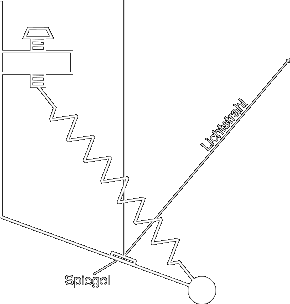
\includegraphics[width=0.6\textwidth]{Figures/Gravity/Exported/Reyko_CCBY-SA_LaCoste-Romberg_Reversed.png}
      
        \small Springconstant \& Extension.
      \end{center}
    \end{PointSix}
\end{frame}


\begin{frame}
  \begin{PointSix}{Pendulum-based gravimeters}
    
    \begin{center}
      \begin{tikzpicture}[font=\footnotesize]
        % Support
        \fill (-1.5,0) rectangle(1.5,0.1);

        % Bob's trajectory
        \draw[dashed] (-60:4) arc(-60:-120:4);

        % Rod + Bob
        \draw (0,0) -- (-60:4) node[fill,circle](m){};

        % Weight Force
        \draw[-latex] (m) -- node[right]{$\vec{g}$}++(0,-1) ;

        % Tension Force
        %\draw [-latex] (m) -- node[right]{$\vec{T}$}(-60:3);

        % Light gray pendulum
        \draw[black!10] (0,0) -- (-90:4) node[fill,circle]{};
        \draw[black!10] (0,0) -- (-120:4) node[fill,circle]{};
        \draw[<->,Karminrot] (0,0) -- (-90:4) node[midway,right]{l};
      \end{tikzpicture}

      Eigenfrequency \& Length.
      $$
      \omega = \sqrt{\frac{g}{l}}
      $$
    \end{center}
  \end{PointSix}
\end{frame}

\begin{frame}
  \begin{PointSix}{Free-fall gravimeters ($\rightarrow$ Ex.)}
      \tiny [FG Gravimeter from MicroGLaCoste]
    \begin{center}
      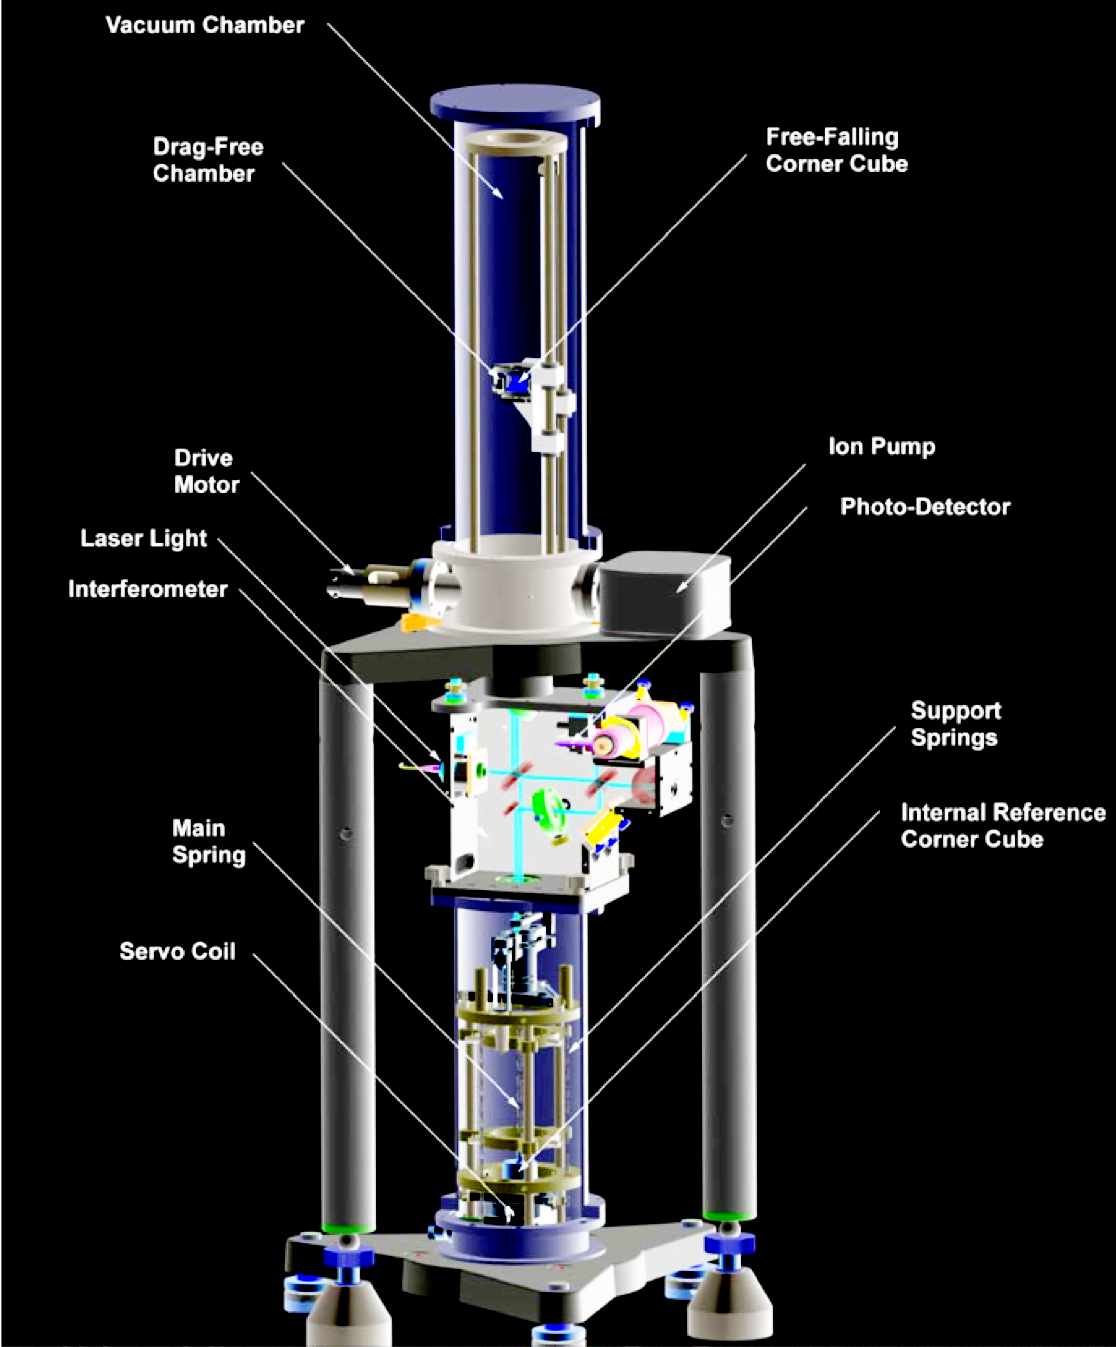
\includegraphics[width=0.55\textwidth]{Figures/Gravity/Exported/FG_Gravimeter_MicroGLaCoste_Reversed.png}

      \small Traveltime \& Distance.
    \end{center}
  \end{PointSix}
\end{frame}

\begin{frame}
  \begin{PointSix}{Gravimeters}
    \begin{itemize}
      \item Unit used is \textit{Gal} (=0.01 ms$^{-2}$)
      \item Top \textit{absolute} gravimeters $\sim 1 \mu$Gal ($10^{-9} g$)
      \item Top \textit{relative} gravimeters $\sim 10 \mu$Gal ($10^{-9} g$)
      \item Typically only $g_z$ is measured.
    \end{itemize}
  \end{PointSix}
\end{frame}
\begin{frame}
    \begin{PointSix}{Instrument drift / temporal variability}
      \resizebox{9 cm}{!}{     
              \begin{tikzpicture}[background rectangle/.style={fill=black},show background rectangle]
                \coordinate (TL) at (-2,-3);
                \coordinate (TR) at (9,-3);
                \coordinate (BL) at (-2,-10);
                \coordinate (BR) at (9,-10);
                \coordinate (Target) at (3.5,-5);

     

                \draw [->,thick,white] (TL) -- (TR) node[circle,fill=Karminrot,pos=0]{A} node[circle,fill=Karminrot,pos=0.2]{B} node[circle,fill=Karminrot,pos=0.4]{C} node[circle,fill=Karminrot,pos=0.6]{D} node[circle,fill=Karminrot,pos=0.8]{E} node[circle,fill=Karminrot,pos=1.0]{F};
                \fill[Karminrot] (Target) circle (2.5ex);
                %\draw[ultra thick,MyBlue] (-1.4,1.3) circle (2.5ex);
                %\draw [<-,line width=1.25mm,MyBlue]  (TL) to[out=30,in=150] (TR);
                \begin{axis}[
                    ylabel={Gravity Anomaly},
                    xlabel={Horizontal Distance},
                    label style={font=\small},
                    axis lines=middle, xtick=\empty,ytick=\empty,
                    color=white,
                    width=12cm,
                    height=\axisdefaultheight,
                    at={(-0.18\linewidth,0)},
                    axis line style=ultra thick,
                    x label style={at={(axis description cs:0.91,-0.025)},anchor=north},
                    y label style={at={(axis description cs:0.91,0.9)},anchor=north}
                      ]
                    \addplot[domain=-80:80,samples=200,color=Karminrot,line width=1.0mm] {5/((25+x*x)^(0.5)*1000)+x/1000000+1/10000};
                    %\addplot[domain=-80:80,samples=200,color=MyBlue,line width=1.0mm,dashed] {5/((25+x*x)^(0.5)*1000)};
                    %\addplot[domain=-80:-70,samples=200,color=Karminrot,mark=-*,line width=1.0mm,dashed] {x*0.0+3/10000};
                  \end{axis}
              \end{tikzpicture}
      }
    \end{PointSix}
\end{frame}


\begin{frame}
  \begin{PointSix}{Instrument drift / temporal variability}
    \resizebox{9 cm}{!}{     
            \begin{tikzpicture}[background rectangle/.style={fill=black},show background rectangle]
              \coordinate (TL) at (-2,-3);
              \coordinate (TR) at (9,-3);
              \coordinate (BL) at (-2,-10);
              \coordinate (BR) at (9,-10);
              \coordinate (Target) at (3.5,-5);

   

              \draw [->,thick,white] (TL) -- (TR) node[circle,fill=Karminrot,pos=0]{A} node[circle,fill=Karminrot,pos=0.2]{B} node[circle,fill=Karminrot,pos=0.4]{C} node[circle,fill=Karminrot,pos=0.6]{D} node[circle,fill=Karminrot,pos=0.8]{E} node[circle,fill=Karminrot,pos=1.0]{F};
              \fill[Karminrot] (Target) circle (2.5ex);
              \draw[ultra thick,MyBlue] (-1.4,1.3) circle (2.5ex);
              \node[MyBlue] at (-1.4,2.4) {offset};
              \draw [<-,line width=1.25mm,MyBlue]  (TL) to[out=30,in=150] (TR);
              \begin{axis}[
                  ylabel={Gravity Anomaly},
                  xlabel={Horizontal Distance},
                  label style={font=\small},
                  axis lines=middle, xtick=\empty,ytick=\empty,
                  color=white,
                  width=12cm,
                  height=\axisdefaultheight,
                  at={(-0.18\linewidth,0)},
                  axis line style=ultra thick,
                  x label style={at={(axis description cs:0.91,-0.025)},anchor=north},
                  y label style={at={(axis description cs:0.91,0.9)},anchor=north}
                    ]
                  \addplot[domain=-80:80,samples=200,color=Karminrot,line width=1.0mm] {5/((25+x*x)^(0.5)*1000)+x/1000000+1/10000};
                  \addplot[domain=-80:80,samples=200,color=MyBlue,line width=1.0mm,dashed] {5/((25+x*x)^(0.5)*1000)};
                  \addplot[domain=-80:-70,samples=200,color=Karminrot,mark=-*,line width=1.0mm,dashed] {x*0.0+3/10000};
                \end{axis}
            \end{tikzpicture}
    }
  \end{PointSix}
\end{frame}

\begin{frame}
  \begin{PointSix}{Absolute vs. relative}
    Absolute gravimeters are needed
    \begin{itemize}
      \item if loop closure if impossible (e.g. intercontinental surveys),
      \item for long-term changes such as isostatic uplift,
      \item as basestations for relative surveys.
    \end{itemize}
    Relative surveys are always easier to conduct and loop closure can cancel many error sources (e.g., instrument drift).
  \end{PointSix}
\end{frame}

\begin{frame}
  \begin{PointSix}{Reduction of gravity data}
    Every gravity survey measures:
    \begin{itemize}
      \item latitudinal variability,
      \item dependency on elevation,
      \item the surrounding terrain,
      \item excess mass above anomaly,
      \item earth \& ocean tides,
      \item (instr. drift, motion compons.).
      \item \alert{density variability in the subsurface.}
    \end{itemize}
  \end{PointSix}
\end{frame}

\begin{frame}
  \begin{PointSix}{Latitudinal variability ($\rightarrow$ Ex.)}
    \small  Extension to ellipsoid contains the same physics.
    \begin{center}
    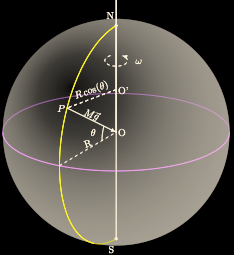
\includegraphics[width=0.5\textwidth]{Figures/Gravity/Exported/GravityFieldEarthRotation_Reversed.png}
    \end{center}
    \small Max 5 Gal (this is large!).
  \end{PointSix}
\end{frame}

\begin{frame}
  \begin{PointSix}{Reduction of gravity data}
    Every gravity survey measures:
    \begin{itemize}
      \item \textcolor{MyBlue}{latitudinal variability},
      \item dependency on elevation,
      \item the surrounding terrain,
      \item excess mass above anomaly,
      \item earth \& ocean tides,
      \item (instr. drift, motion compons.).
      \item \alert{density variability in the subsurface.}
    \end{itemize}
  \end{PointSix}
\end{frame}

\begin{frame}
  \begin{PointSix}{Elevation correction (i.e. free-air)}
    \resizebox{9 cm}{!}{     
            \begin{tikzpicture}[background rectangle/.style={fill=black},show background rectangle]
              \coordinate (TL) at (-2,-3);
              \coordinate (TR) at (9,-3);
              \coordinate (BL) at (-2,-10);
              \coordinate (BR) at (9,-10);
              \coordinate (Target) at (3.5,-5);

   

              \draw [->,thick,white] (TL) -- (TR) node[circle,fill=Karminrot,pos=0]{A} node[circle,fill=Karminrot,pos=0.2]{B} node[circle,fill=Karminrot,pos=0.4]{C} node[circle,fill=Karminrot,pos=0.6]{D} node[circle,fill=Karminrot,pos=0.8]{E} node[circle,fill=Karminrot,pos=1.0]{F};
              \fill[Karminrot] (Target) circle (2.5ex);
              \begin{axis}[
                  ylabel={Gravity Anomaly},
                  xlabel={Horizontal Distance},
                  label style={font=\small},
                  axis lines=middle, xtick=\empty,ytick=\empty,
                  color=white,
                  width=12cm,
                  height=\axisdefaultheight,
                  at={(-0.18\linewidth,0)},
                  axis line style=ultra thick,
                  x label style={at={(axis description cs:0.91,-0.025)},anchor=north},
                  y label style={at={(axis description cs:0.91,0.9)},anchor=north}
                    ]
                 % \addplot[domain=-80:80,samples=200,color=Karminrot,line width=1.0mm] {5/((25+x*x)^(0.5)*1000)+x/1000000+1/10000};
                  \addplot[domain=-80:80,samples=200,color=MyBlue,line width=1.0mm] {5/((25+x*x)^(0.5)*1000)};
                  %\addplot[domain=-80:-70,samples=200,color=Karminrot,mark=-*,line width=1.0mm,dashed] {x*0.0+3/10000};
                \end{axis}
            \end{tikzpicture}
    }
  \end{PointSix}
\end{frame}

\begin{frame}
  \begin{PointSix}{Elevation correction (i.e. free-air)}
    \resizebox{9 cm}{!}{     
            \begin{tikzpicture}[background rectangle/.style={fill=black},show background rectangle]
              \coordinate (TL) at (-2,-2);
              \coordinate (TR) at (9,-2);
              \coordinate (BL) at (-2,-10);
              \coordinate (BR) at (9,-10);
              \coordinate (Target) at (3.5,-5);

   

              \draw [->,thick,white] (TL) -- (TR) node[circle,fill=Karminrot,pos=0]{A} node[circle,fill=Karminrot,pos=0.2]{B} node[circle,fill=Karminrot,pos=0.4]{C} node[circle,fill=Karminrot,pos=0.6]{D} node[circle,fill=Karminrot,pos=0.8]{E} node[circle,fill=Karminrot,pos=1.0]{F};
              \fill[Karminrot] (Target) circle (2.5ex);
              \begin{axis}[
                  ylabel={Gravity Anomaly},
                  xlabel={Horizontal Distance},
                  label style={font=\small},
                  axis lines=middle, xtick=\empty,ytick=\empty,
                  color=white,
                  width=12cm,
                  height=\axisdefaultheight,
                  at={(-0.18\linewidth,0)},
                  axis line style=ultra thick,
                  x label style={at={(axis description cs:0.91,-0.025)},anchor=north},
                  y label style={at={(axis description cs:0.91,0.9)},anchor=north}
                    ]
                 % \addplot[domain=-80:80,samples=200,color=Karminrot,line width=1.0mm] {5/((25+x*x)^(0.5)*1000)+x/1000000+1/10000};
                 \addplot[domain=-80:80,samples=200,color=MyBlue,line width=1.0mm,dashed] {5/((25+x*x)^(0.5)*1000)};
                  \addplot[domain=-80:80,samples=200,color=MyBlue,line width=1.0mm] {0.6*5/((25+x*x)^(0.5)*1000)};
                  %\addplot[domain=-80:-70,samples=200,color=Karminrot,mark=-*,line width=1.0mm,dashed] {x*0.0+3/10000};
                \end{axis}
            \end{tikzpicture}
    }
  \end{PointSix}
\end{frame}

\begin{frame}
  \begin{PointSix}{Elevation correction}
    The elevation correction references the gravity anomaly to the same datum (e.g., the geoid). 
    
    \alert{How does the gravitational acceleration change with elevation near the Earth's surface?}
  \end{PointSix}
\end{frame}

\begin{frame}
  \begin{PointSix}{Elevation correction via Taylor expansion}
    Taylor expansion near $r=R_E$:
    \only<1>
    {
      $$
        g(r) = g(R_E) + \frac{dg}{dr}|_{R_E}
      $$
    }
    \only<2>
    {
      $$
        g(r) \approx G\frac{M}{R_E^2} - 2G\frac{M}{R_E^3}(r-R_E) + ...
      $$
    }
    \only<3>
    {
      $$
        g(r) \approx \underbrace{G\frac{M}{R_E^2}}_{\text{g at Earth's surface}} - 2G\frac{M}{R_E^3}(r-R_E) + ...
      $$
    }
    \only<4>
    {
      $$
        g(r) \approx G\frac{M}{R_E^2} - \underbrace{2G\frac{M}{R_E^3}(r-R_E)}_{\text{change with elevation}} + ...
      $$
    }
    \only<5>
    {
      $$
        g(r) \approx G\frac{M}{R_E^2} - \underbrace{2G\frac{M}{R_E^3}(r-R_E)}_{\text{change with elevation}} + ...
      $$
      Evaluation at let's say $r=R_E+1$ (m) returns a change of $\delta g(r)\approx -0.3$ mGal per m.
    }
    \only<6>
    {
      $$
        g(r) \approx G\frac{M}{R_E^2} - \underbrace{2G\frac{M}{R_E^3}(r-R_E)}_{\text{change with elevation}} + ...
      $$
      $\delta g(r)\approx -0.3$ mGal per m is large compared to the sensitivity of gravimeters, \alert{therefore the gravimeter elevation needs to be determined within centimeters using GNSS.}
    }
  \end{PointSix}
\end{frame}

\begin{frame}
  \begin{PointSix}{Reduction of gravity data}
    Every gravity survey measures:
    \begin{itemize}
      \item \textcolor{MyBlue}{latitudinal variability},
      \item \textcolor{MyBlue}{dependency on elevation},
      \item the surrounding terrain,
      \item excess mass above anomaly,
      \item earth \& ocean tides,
      \item (instr. drift, motion compons.).
      \item \alert{density variability in the subsurface.}
    \end{itemize}
  \end{PointSix}
\end{frame}

\begin{frame}
  \begin{PointSix}{Reduction of gravity data: Terrain correction}
   \begin{tikzpicture}
      \coordinate (TL) at (-2,-2);
      \coordinate (TR) at (9,-2);
      \coordinate (BL) at (-2,-10);
      \coordinate (BR) at (9,-10);
      \coordinate (Target) at (3.5,-3);

      \draw [->,thick,white] ([xshift=4cm,yshift=2cm] TL) -- ([yshift=2cm] TR);
      %\draw [->,thick,white,dashed] (TL) -- (TR) node[draw=none,fill=none,font=\scriptsize,near start,below] {reference surface};
      %\draw ([yshift=2cm] TL) .. controls ([xshift=2cm,yshift=4cm] TL) .. ([xshift=4.0cm,yshift=2cm] TL) ;
      \draw ([yshift=2cm] TL) ([xshift=4.0cm,yshift=2cm] TL) ;
      \fill[Karminrot] (Target) circle (2.5ex);
      %\draw [->, line width=1.5mm](3.5,0) -- (2.7,-1.7);
      \draw [->, line width=1.5mm,dashed](3.5,0) -- (3.5,-2);
     %\draw [line width=1.0mm,dashed](2.7,-1.7) -- (0,1) node[draw=none,fill=none,font=\small,midway,below,rotate=-46] {mass excess};
   \end{tikzpicture}
  \end{PointSix}
\end{frame}


\begin{frame}
  \begin{PointSix}{Reduction of gravity data: Terrain correction}
   \begin{tikzpicture}
      \coordinate (TL) at (-2,-2);
      \coordinate (TR) at (9,-2);
      \coordinate (BL) at (-2,-10);
      \coordinate (BR) at (9,-10);
      \coordinate (Target) at (3.5,-3);

      \draw [->,thick,white] ([xshift=4cm,yshift=2cm] TL) -- ([yshift=2cm] TR);
      %\draw [->,thick,white,dashed] (TL) -- (TR) node[draw=none,fill=none,font=\scriptsize,near start,below] {reference surface};
      \draw ([yshift=2cm] TL) .. controls ([xshift=2cm,yshift=4cm] TL) .. ([xshift=4.0cm,yshift=2cm] TL) ;
      \fill[Karminrot] (Target) circle (2.5ex);
      \draw [->, line width=1.5mm](3.5,0) -- (2.7,-2);
      \draw [->, line width=1.5mm,dashed](3.5,0) -- (3.5,-2);
      \draw [line width=1.0mm,dashed](2.7,-2) -- (0,1) node[draw=none,fill=none,font=\small,midway,below,rotate=-46] {mass excess};
   \end{tikzpicture}
  A neighboring mountain will reduce the measured $g_z$ independent of target properties.
  \end{PointSix}
\end{frame}
\begin{frame}
  \begin{PointSix}{Reduction of gravity data: Terrain correction}
   \begin{tikzpicture}
      \coordinate (TL) at (-2,-2);
      \coordinate (TR) at (9,-2);
      \coordinate (BL) at (-2,-10);
      \coordinate (BR) at (9,-10);
      \coordinate (Target) at (3.5,-3);

      \draw [->,thick,white] ([xshift=4cm,yshift=2cm] TL) -- ([yshift=2cm] TR);
      %\draw [->,thick,white,dashed] (TL) -- (TR) node[draw=none,fill=none,font=\scriptsize,near start,below] {reference surface};
      \draw ([yshift=2cm] TL) .. controls ([xshift=2cm,yshift=0cm] TL) .. ([xshift=4.0cm,yshift=2cm] TL) ;
      \fill[Karminrot] (Target) circle (2.5ex);
      \draw [->, line width=1.5mm](3.5,0) -- (4.3,-2);
      \draw [->, line width=1.5mm,dashed](3.5,0) -- (3.5,-2);
      \draw [line width=1.0mm,dashed](3.5,-2) -- (0,-1) node[draw=none,fill=none,font=\small,midway,below,rotate=-20] {mass deficit};
   \end{tikzpicture}
  A neighboring valley will reduce the measured $g_z$ independent of target properties.
  \end{PointSix}
\end{frame}

\begin{frame}
  \begin{PointSix}{Reduction of gravity data: Terrain correction}
  \begin{itemize}
    \item The terrain correction requires an elevation model and assumptions about the broad-scale sub-surface density.
    \item The terrain correction is positive both for surrounding valleys and mountains.
  \end{itemize}
\end{PointSix}
\end{frame}

\begin{frame}
  \begin{PointSix}{Reduction of gravity data}
    Every gravity survey measures:
    \begin{itemize}
      \item \textcolor{MyBlue}{latitudinal variability},
      \item \textcolor{MyBlue}{dependency on elevation},
      \item \textcolor{MyBlue}{the surrounding terrain},
      \item excess mass above anomaly,
      \item earth \& ocean tides,
      \item (instr. drift, motion compons.).
      \item \alert{density variability in the subsurface.}
    \end{itemize}
  \end{PointSix}
\end{frame}

\begin{frame}
  \begin{PointSix}{Reduction of gravity data: Terrain correction}
   \begin{tikzpicture}
      \coordinate (TL) at (-2,-2);
      \coordinate (TR) at (9,-2);
      \coordinate (BL) at (-2,-10);
      \coordinate (BR) at (9,-10);
      \coordinate (Target) at (3.5,-3);

      \draw [->,thick,white] ([xshift=4cm,yshift=2cm] TL) -- ([yshift=2cm] TR);
      \draw [->,thick,white,dashed] (TL) -- (TR) node[draw=none,fill=none,font=\scriptsize,near start,below] {reference surface};
      \draw ([yshift=2cm] TL) .. controls ([xshift=2cm,yshift=4cm] TL) .. ([xshift=4.0cm,yshift=2cm] TL) ;
      \fill[Karminrot] (Target) circle (2.5ex);
      \draw [->, line width=1.5mm,Karminrot](3.5,0) -- (3.5,-1);

   \end{tikzpicture}
  \small Elevation and terrain correction to not account for the mass between the measurement surface and the reference surface.
  \end{PointSix}
\end{frame}

\begin{frame}
  \begin{PointSix}{Reduction of gravity data: Terrain correction}
   \begin{tikzpicture}
      \coordinate (TL) at (-2,-2);
      \coordinate (TR) at (9,-2);
      \coordinate (BL) at (-2,-10);
      \coordinate (BR) at (9,-10);
      \coordinate (Target) at (3.5,-3);

      %\draw [->,thick,white] ([xshift=4cm,yshift=2cm] TL) -- ([yshift=2cm] TR);
      %\draw [->,thick,green,name path = A] ([yshift=2cm] TL) -- ([yshift=2cm] TR);
      \draw [->,thick,white,dashed,name path = B] (TL) -- (TR) node[draw=none,fill=none,font=\scriptsize,near start,below] {reference surface};
      \draw ([yshift=2cm] TL) .. controls ([xshift=2cm,yshift=4cm] TL) .. ([xshift=4.0cm,yshift=2cm] TL) ;
      \fill[Karminrot] (Target) circle (2.5ex);
      \fill[pattern=north west lines,pattern color=white] ([yshift=2cm] TL) rectangle (TR);
      \draw [->, line width=1.5mm,Karminrot](3.5,0) -- (3.5,-1);
      \draw [|-|, line width=0.5mm,white]([xshift=-0.5cm] TL) -- ([xshift=-0.5cm, yshift=2cm] TL) node[draw=none,fill=none,font=\scriptsize,midway,left] {h};;
      
   \end{tikzpicture}
  \only<1>{
    \small What is the effect $\delta g_z$ of a horizontal plate with constant density?
  }
  \only<2>{
    \small $g_z = G \rho \int \int \int \frac{1}{r^2}\cos(\phi) dV = ? $
  }
  \only<3>{
    \small $g_z = G \rho \int \int \int \frac{1}{r^2}\cos(\phi) dV = 2\pi G\rho h$
  }
  \end{PointSix}
\end{frame}
\begin{frame}
  \begin{PointSix}{Reduction of gravity data}
    Every gravity survey measures:
    \begin{itemize}
      \item \textcolor{MyBlue}{latitudinal variability},
      \item \textcolor{MyBlue}{dependency on elevation},
      \item \textcolor{MyBlue}{the surrounding terrain},
      \item \textcolor{MyBlue}{excess mass above anomaly},
      \item earth \& ocean tides,
      \item (instr. drift, motion compensation),
      \item \alert{density variability in the subsurface.}
    \end{itemize}
  \end{PointSix}
\end{frame}

\begin{frame}
  \begin{PointSix}{The origin of tides}
      \begin{itemize}
        \item Tides are caused by gravity celestial bodies (i.e. Sun \& Moon).
        \item Tidal forces vary across a spatially extended body.
        \item Tidal forces are balanced by centrifugal forces of two (three) body rotations.
      \end{itemize}
  \end{PointSix}
\end{frame}

\begin{frame}
  \begin{PointSix}{The origin of tides}
  \begin{tikzpicture}
    \coordinate (EC) at (5,0) node[yshift=-2cm,draw=none,fill=none,font=\small,below] {Earth};
    \coordinate (MC) at (0,0) node[yshift=-2cm,xshift=5cm,draw=none,fill=none,font=\small,below] {Moon};
    \fill[white] (EC) circle (4.5ex);
    \fill[white] (MC) circle (1.5ex);
    %§\draw [->, line width=1.5mm,Karminrot](EC) -- (MC);
    % \begin{axis}[
    %   ylabel={F},
    %   xlabel={distance r},
    %   label style={font=\tiny},
    %   axis lines=middle, xtick=\empty,ytick=\empty,
    %   color=Karminrot,
    %   width=8cm,
    %   height=4cm,
    %   ymin=0.0,
    %   %ymax=5.16,
    %   at={(0.0\linewidth,0.0\linewidth)},
    %   axis line style=ultra thick,
    %   x label style={at={(axis description cs:0.4,-0.025)},anchor=north},
    %   y label style={at={(axis description cs:-0.1,0.9)},anchor=north}
    %     ]

    %  \addplot[domain=0.6:1.5,samples=200,color=MyBlue,line width=1.0mm,dashed] {1/(x*x))};
    % \end{axis}
  \end{tikzpicture}
  \end{PointSix}
\end{frame}

\begin{frame}
  \begin{PointSix}{The origin of tides}
  \begin{tikzpicture}
    \coordinate (EC) at (5,0) node[yshift=-2cm,draw=none,fill=none,font=\small,below] {Moon};
    \coordinate (MC) at (0,0) node[yshift=-2cm,xshift=5cm,draw=none,fill=none,font=\small,below] {Earth};
    \fill[white] (EC) circle (4.5ex);
    \fill[white] (MC) circle (1.5ex);
    %§\draw [->, line width=1.5mm,Karminrot](EC) -- (MC);
    \begin{axis}[
      ylabel={F},
      xlabel={distance r},
      label style={font=\tiny},
      axis lines=middle, xtick=\empty,ytick=\empty,
      color=Karminrot,
      width=8cm,
      height=4cm,
      ymin=0.0,
      %ymax=5.16,
      at={(0.0\linewidth,0.0\linewidth)},
      axis line style=ultra thick,
      x label style={at={(axis description cs:0.4,-0.025)},anchor=north},
      y label style={at={(axis description cs:-0.1,0.9)},anchor=north}
        ]

     \addplot[domain=0.6:1.5,samples=200,color=MyBlue,line width=1.0mm,dashed] {1/(x*x))};
    \end{axis}
  \end{tikzpicture}
  \vspace{1cm}

  \small Gravitational attraction is stronger on the nearside than the farside.
  \end{PointSix}
\end{frame}

\begin{frame}
  \begin{PointSix}{The origin of tides}
    \begin{tikzpicture}
        \coordinate (EC) at (5,0);
        \coordinate (MC) at (0,0);
        \coordinate (RP) at (4,0);
        \fill[white] (EC) circle (4.5ex) node[yshift=-2cm,draw=none,fill=none,font=\small,below] {Earth};
        \fill[white] (MC) circle (1.5ex) node[yshift=-2cm,draw=none,fill=none,font=\small,below] {Moon};
        \fill[Karminrot] (RP) circle (0.5ex);
        \draw [->,thick,Karminrot] (RP) -- ([yshift=2cm] RP) node [midway] {\AxisRotator[rotate=-90]};
        \draw [|-|,thick,Karminrot] (EC) -- (MC);
   \end{tikzpicture}
   
          \pause
          \small Centrifugal force can be projected into radial (i.e. parallel to Earth's gravitation) and parallel component. This leads to the force balance.
  \end{PointSix}
\end{frame}

\begin{frame}
  \begin{PointSix}{The origin of tides}
  \begin{tikzpicture}
    \coordinate (RP) at (1,0);
    \node[inner sep=0pt] (russell) at (0,0)
      {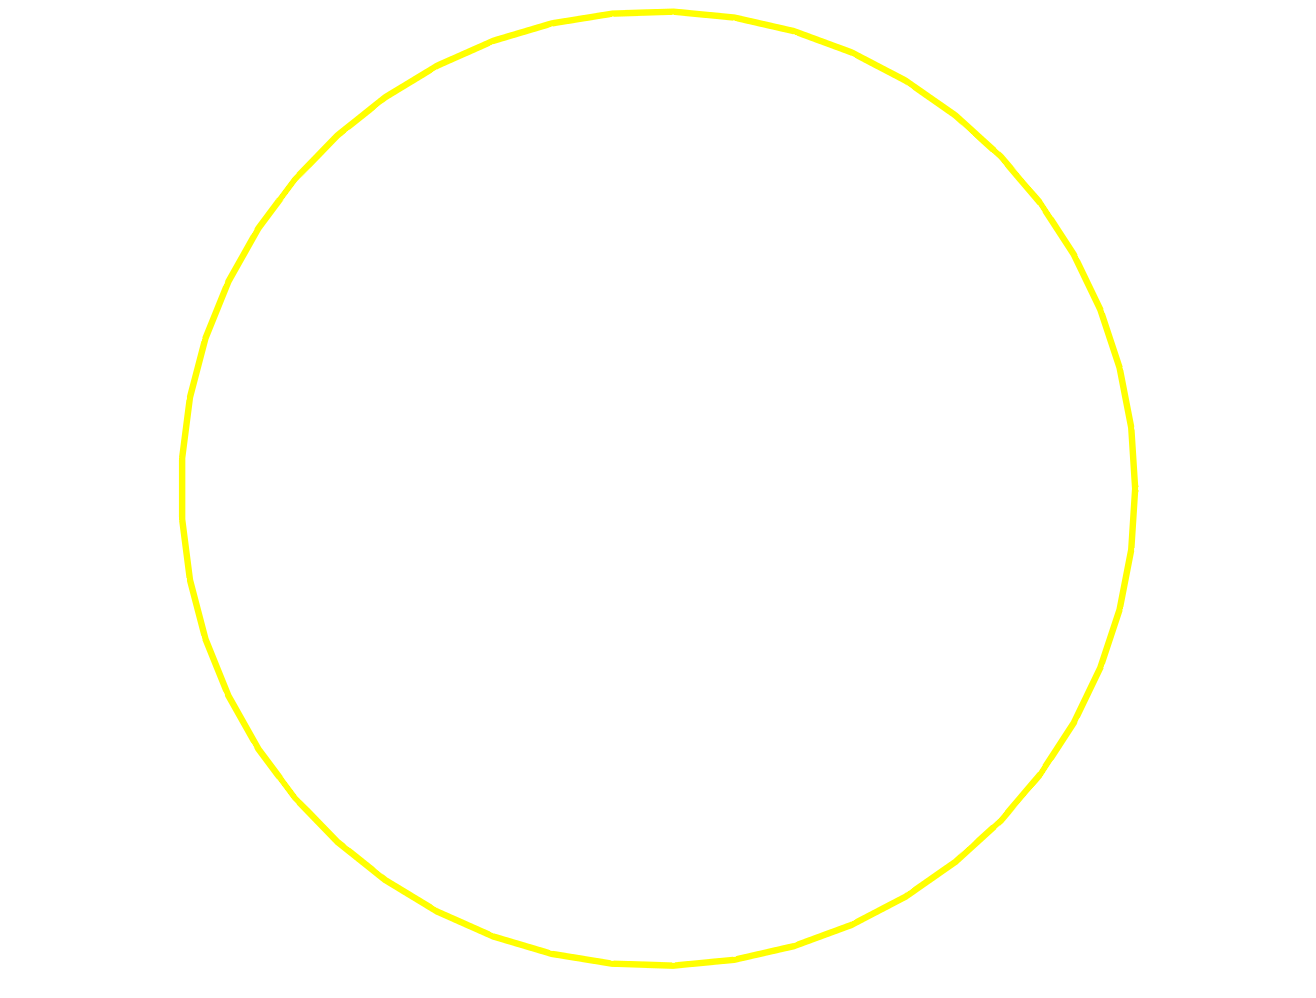
\includegraphics[width=.6\textwidth]{Figures/Gravity/Exported/Field_tidal.png}};
      \fill[white] (5,0) circle (1.5ex) node[yshift=-2cm,draw=none,fill=none,font=\small,below] {Moon};
      \draw [->,thick,Karminrot] (RP) -- ([yshift=2cm] RP) node [midway] {\AxisRotator[rotate=-90]};
      \draw [|-|,thick,Karminrot] (RP) -- (5,0);
  \end{tikzpicture}
  \small The lunar gravity differential field is responsible for two tidal bulges (i.e. tides twice a day).
\end{PointSix}
\end{frame}

\begin{frame}
  \begin{PointSix}{The origin of tides}
      \small
      \begin{itemize}
        \item Tidal forces vary across a spatially extended body.
        \item Tidal forces are balanced by centrifugal forces of two (three) body rotations.
        \item There is lots of confusion regarding the origin of tides (cf. Matsuda et al. 2015 $\rightarrow$ Ilias).
        \item \color{MyBlue}{Tide models can be used for correction} 
      \end{itemize}
  \end{PointSix}
\end{frame}

\begin{frame}
  \begin{PointSix}{Reduction of gravity data}
    Every gravity survey measures:
    \begin{itemize}
      \item \textcolor{MyBlue}{latitudinal variability},
      \item \textcolor{MyBlue}{dependency on elevation},
      \item \textcolor{MyBlue}{the surrounding terrain},
      \item \textcolor{MyBlue}{excess mass above anomaly},
      \item \textcolor{MyBlue}{earth \& ocean tides},
      \item (instr. drift, motion compensation),
      \item \alert{density variability in the subsurface.}
    \end{itemize}
  \end{PointSix}
\end{frame}

\begin{frame}
  \begin{PointSix}{Reduction of gravity data}
    Every gravity survey measures:
    \begin{itemize}
      \item \textcolor{MyBlue}{latitudinal variability},
      \item \textcolor{MyBlue}{dependency on elevation},
      \item \textcolor{MyBlue}{the surrounding terrain},
      \item \textcolor{MyBlue}{excess mass above anomaly},
      \item \textcolor{MyBlue}{earth \& ocean tides},
      \item \textcolor{MyBlue}{(instr. drift, motion compensation)},
      \item \alert{density variability in the subsurface.}
    \end{itemize}
  \end{PointSix}
\end{frame}